This chapter introduces the theory of anyons by a set of physical requirements.
The algebraic definition of anyons will then by given by the discussion in
\Cref{sect:Categories}.

Anyons are proposed as a \emph{defect} in a $2$ dimensional space (manifold?
compact?) with \emph{exotic exchange statistics}. These exchange statistics
differ from bosons or fermions in that we allow particles to pick up a arbitrary
phase $e^{i\theta}$ on exchange in the abelian case, and a phase as a matrix
element in the nonabelian case.

We group anyons into theories. An anyon theory carries a finite set of charges
(types) $a,b,c\ldots$ including a trivial \emph{vacuum} charge. We are then
interested in their spacetime histories, as this is where the topological
properties of the anyon become apparent. First fix an oriented manifold $D$ of
dimension two as our base space. Then introduce an anyonic defect as a point
like hole (that is also oriented), that is carrying a charge. Such a particles
spacetime history is then given by an appropriate 3-manifold.\todo{I dont like
this whole section.}

\section{Configuration Spaces \& The Braid Group}
\label{sect:anyons1:configurations_spaces_and_the_braid_group}

The original article by \textcite{leinaasTheoryIdenticalParticles1977a}
identifies a generalized theory of \emph{identical} particles. Denote the space
where a particle lives by $\Sigma$ and thus the space of $n$ particles possible
coordinates of equal type by $\Sigma^n$. Since the particles are assumed to be
identical, any permutation (an action of $S_n$) necessarily leads to the same
physical state, so we denote the full space of our system by the quotient
\[
    \Sigma^n / S_n.
\] 
However we also want no two particles occupying the same space\footnote{If this
were the case, then the resulting exchange statistics would be bosonic
\cite[Footnote~12]{wuGeneralTheoryQuantum1984}.}, so the diagonal in $\Delta =
\{x \in \Sigma^n \mid x_i = x_j \text{ for some } i \neq j\}$\todo{rephrase!}
needs to be excluded as well \cite{wuGeneralTheoryQuantum1984}. This leads to the expression
\[
    \uConf_n(\Sigma) = (\Sigma^n - \Delta) / S_n
\]  
which is defined to be the \emph{configuration space} of $n$ unordered
particles. However as we will see, anyons come in different "types", and we
consider only particles of the same type to be identical. Later publications
however define a swath of different notions of configuration spaces. We follow
\cite{satiDifferentialCohomotopyImplies2022}\todo{original publications.} with
the following definition:
\begin{definition}
    The \emph{\green{ordered Configuration Space}} of $n$ particles of possibly
    differnt types (or labeled particles with the same type) on a surface of
    dimension $D$ is
    \[
        \oConf n (\Sigma) := (\Sigma)^n - \Delta_{\Sigma}^n
    \] 
    and the \emph{\green{unordered Configuration Space}} of $n$ unlabeled
    identical particles is defined as 
    \[
        \uConf_n (\Sigma) := \oConf n (\Sigma) / S_n.
    \]
\end{definition}    

\begin{figure}
  \includegraphics[width=0.5\textwidth]{figures/conf_5.png}
  \caption{The configuration space of 5 particles in the plane $\R^2$.}
\end{figure}

Note that while \cite{leinaasTheoryIdenticalParticles1977a} conjectured
computations for strange exchange statistics in both $2$ and $3$ dimensions, the
concept of an anyon as a $1$ dimensional representation is due to
\cite{wilczek1990}. 

Now we want to classify all the possible motions particles can take in this
space. The \emph{motion group} of the configuration space is given by the spaces
\emph{homotopy classes} (c.f. \Cref{app_gen:homotopy}), which are given by the
fundamental group(oid) of the spcae. Informally, this group collects all the
loops at some configuration $x_0$ up to homotopy. We want to differentiate two
cases here: If $D = 2$ it is known that

\[
    \pi_1(\uConf_n (\Sigma)) = \Br_n(\Sigma) \quad \text{ and } \quad \pi_1(\oConf{n} (\Sigma)) = \PBr_n(\Sigma)
\]
however if $D >= 3$ we know that both of these coincide with the symmetric group
$S_n$ instead. In fact there is an exact sequence
\[
    1 
    \longrightarrow 
    \mathrm{PBr}_n(\Sigma) 
    \longrightarrow 
    \mathrm{Br}_n(\Sigma)
    \longrightarrow 
    S_n 
    \longrightarrow 
    1 .
\]
For an example in the plane $\R^2$ (or $\C$?), we give an explicit
representation of the \emph{braid group} $\Br_n(\R^2)$ and the \emph{pure braid
group} $\PBr_n(\R^2)$. There is a well know presentation in terms of generators
due to \cite{artin25} as
\[
    \Br_n(\R^2)
    = 
    \left\langle
    \sigma_1, \ldots, \sigma_{n-1}
    \;\middle\vert\;
    \begin{aligned}
        \sigma_i\sigma_{i+1}\sigma_i &= \sigma_{i+1}\sigma_i \sigma_{i+1} \\
        \sigma_i\sigma_j &= \sigma_j\sigma_i,\; \vert i - j \vert \geq 2
    \end{aligned}
    \right\rangle.
\]
These generators also have a graphical interpretation as
\begin{equation}
\sigma_i
\;\coloneqq\;
\left[
\color{black}
\raisebox{-28pt}{
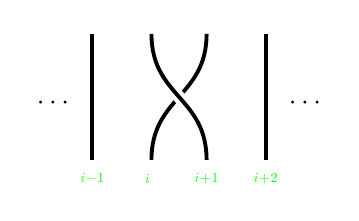
\begin{tikzpicture}[yscale=.8]

\begin{scope}[shift={(-1.6,0)}]
\draw[line width=1.4]
  (+.5,1) to (+.5,-1);
\draw
  (-0,-.1) node {$\mathclap{\cdots}$};
\end{scope}
\draw[line width=1.4]
  (-.35,-1)
  .. controls (-.35,0) and (+.35,0)  ..
  (+.35,1);

\draw[line width=4.5, white]
  (+.35,-1)
  .. controls (+.35,0) and (-.35,0)  ..
  (-.35,1);
\draw[line width=1.4]
  (+.35,-1)
  .. controls (+.35,0) and (-.35,0)  ..
  (-.35,1);
\begin{scope}[shift={(+1.6,0)}]
\draw[line width=1.4]
  (-.5,1) to (-.5,-1);
\draw
  (-0,-.1) node {$\mathclap{\cdots}$};
\end{scope}

\draw
  (-1.1, -1.3) node {\color{green}\scalebox{.5}{$i\!-\!1$}};
\draw
  (-.4, -1.3) node {\color{green}\scalebox{.5}{$i$}};
\draw
  (+.35, -1.3) node {\color{green}\scalebox{.5}{$i\!+\!1$}};
\draw
  (+1.1, -1.3) node {\color{green}\scalebox{.5}{$i\!+\!2$}};
\end{tikzpicture}
} 
\right]
\end{equation}

Now we can give a process as the \emph{spacetime history} diagram of the $n$ particles.

    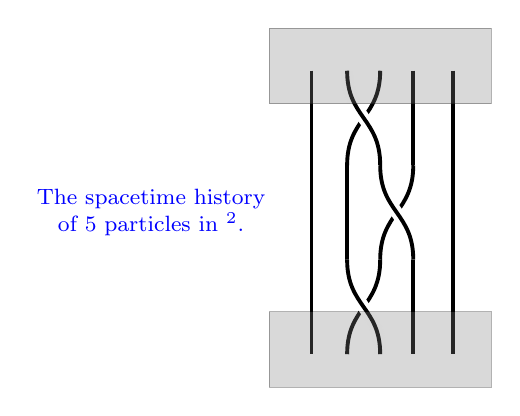
\begin{tikzpicture}
\begin{scope}[scale=0.6]
  \begin{scope}[shift={(-1.6,0)}]
    \draw[line width=1.2]
      (+.5,5) to (+.5,-1);
  \end{scope}

  \begin{scope}[shift={(0,4)}]
    \draw[line width=1.4]
      (-.35,-1)
      .. controls (-.35,0) and (+.35,0)  ..
      (+.35,1);

    \draw[line width=4.5, white]
      (+.35,-1)
      .. controls (+.35,0) and (-.35,0)  ..
      (-.35,1);
    \draw[line width=1.4]
      (+.35,-1)
      .. controls (+.35,0) and (-.35,0)  ..
      (-.35,1);
  \end{scope}

  \draw[line width=1.4]
    (-.35,3)
    --
    (-.35,1);

  \draw[line width=1.4]
    (+1.05,5)
    --
    (+1.05,3);

  \begin{scope}[shift={(.7,2)}]
    \draw[line width=1.4]
      (-.35,-1)
      .. controls (-.35,0) and (+.35,0)  ..
      (+.35,1);

    \draw[line width=4.5, white]
      (+.35,-1)
      .. controls (+.35,0) and (-.35,0)  ..
      (-.35,1);
    \draw[line width=1.4]
      (+.35,-1)
      .. controls (+.35,0) and (-.35,0)  ..
      (-.35,1);
  \end{scope}

  \begin{scope}
    \draw[line width=1.4]
      (-.35,-1)
      .. controls (-.35,0) and (+.35,0)  ..
      (+.35,1);

    \draw[line width=4.5, white]
      (+.35,-1)
      .. controls (+.35,0) and (-.35,0)  ..
      (-.35,1);
    \draw[line width=1.4]
      (+.35,-1)
      .. controls (+.35,0) and (-.35,0)  ..
      (-.35,1);
  \end{scope}

  \draw[line width=1.4]
    (1.05,1) to (1.05,-1);

  \begin{scope}[shift={(+2.4,0)}]
    \draw[line width=1.4]
      (-.5,5) to (-.5,-1);
  \end{scope}

  \draw[fill=gray, opacity=0.3] (-2,4.3) rectangle (2.7,5.9);

  \draw[fill=gray, opacity=0.3] (-2,-0.1) rectangle (2.7,-1.7);

  \node[align=center, blue, font=\footnotesize] at (-4.5, 2) 
        {The spacetime history \\ of $5$ particles in $\R^2$.};

  \end{scope}
\end{tikzpicture}

Now, if we associate a Hilbert space to this configuration space, we can achieve
this by using a \emph{Hilbert Bundle}
\[
  \mathcal{H} \overset{\pi}{\longrightarrow} \oConf{n}(\Sigma),
\]
i.e. to each point $x \in \oConf{n}(\Sigma)$ there is an associated Hilbert
space $\mathcal{H}_{x}$. Furthermore, a path through the configuration space
$[\gamma] : x_0 \to x_1 \in \oConf{n}(\Sigma)$ is lifted to some unitary
representation
\[
  \rho([\gamma]) \in U(\mathcal{H}_{x_0} \to \mathcal{H}_{x_1})
\]
by \emph{parallel transport}.

The closed paths in the respective groups form a \emph{monodromy} in the
configuration space and a \emph{holonomy} in the Hilbert Bundle.


However, in the usual literature anyons are also identified over their
\emph{fusion tensor category} (c.f. \Cref{sect:Categories}). Shifting the
viewpoint from configuration spaces to fusion categories requires additional
postulates \todo{is this true?} about the systems we want to reason about.
Although this correspondence is well known and the categorical interpretation
can be considered standard, a formal treatment and proof \todo{Check if htis is
a full proof.} were only given recently. These are pointed out in
\cite{valeraFusionStructureExchange2021}, and formally rigorous derivations of
this fact are given in \cite{satiAnyonicTopologicalOrder2023}. However we will
not give a derivation of this result and instead assume it. Perhaps a more
natural introduction to this correspondence is given by an excursion over MCGs
as done in \cite{burtonShortGuideAnyons2016}.